\documentclass[12pt]{article}
\usepackage[margin=1.5cm]{geometry}
\usepackage{parskip}
\usepackage{amsmath}
\usepackage{amssymb}
\usepackage{amsfonts}
\usepackage{enumitem}
\usepackage{graphicx}
\usepackage{stmaryrd}
\graphicspath{ {./images/} }


\begin{document}
\begin{enumerate}[label=(\alph*)]

  \item
    \begin{enumerate}[label=(\roman*)]

      \item

        To calculate $P_{TT}$ we need to calculate $\frac{N_{TT}}{\sum_{X \in \{T,C,A,G\}} N_{TX}} = \frac{306}{774} = \frac{17}{43}$

        To calculate $P_{AG}$, we calculate $\frac{N_{AG}}{\sum_{X \in \{T,C,A,G\}} N_{AX}} = \frac{126}{600} = \frac{21}{100}$.

      \item
        $P_{TT}$ and $P_{AG}$ in the complementary sequence is equal to $P_{AA}$ and $P_{TC}$ in the original sequence.

        We calculate the probabilities with the same method as before:

        $P_{TT} = P_{AA} = \frac{11}{50}$

        $P_{AG} = P_{TC} = \frac{38}{129}$.

    \end{enumerate}

  \item
    We begin with each species in its own cluster.

    Clearly, the two closest clusters are $\{A\}$ and $\{B\}$, so we join them.

    This creates the following distance matrix:

    \begin{tabular}{cccc}
      &\{A,B\}&C&D\\
      \{A,B\}&&0.38&0.365\\ 
      C&&&0.44\\
      D&\\
    \end{tabular}

    The two closest clusters are then $\{A,B\}$ and $\{D\}$, so we join them.

    Then, we have no choice but to join $\{A,B,D\}$ and $\{C\}$.

    This yields the following tree:


    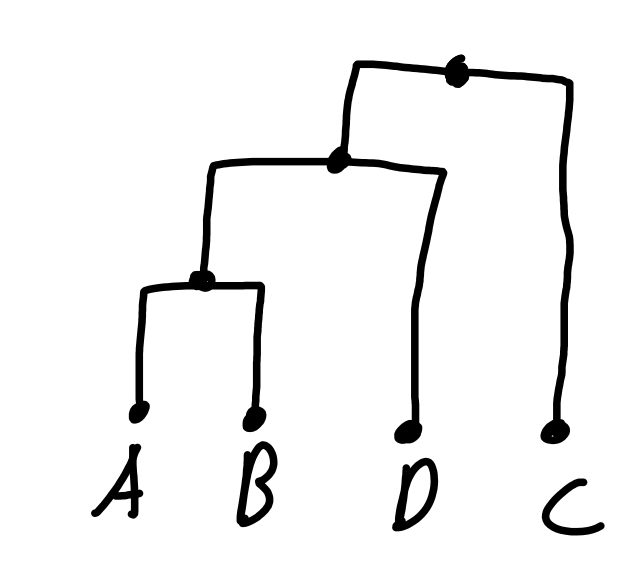
\includegraphics[scale=0.3]{upgma}

  \item
    To build an HMM to predict secondary structure, we need to decide on what the emissions represent, and what the hidden states represent.

    For predicting protein secondary structure, we want the secondary structure to be our hidden states (such that we can predict them with decoding), and the emissions to be something easily observable, like the amino acids. Then, a sequence of emissions represents a protein, as an amino acid sequence. The hidden state at a particular point in the sequence is then the structure of the protein at that point.

    If we had a transition probability matrix and an emission probability matrix, we could then predict protein secondary structure from an amino acid sequence using a decoding algorithm (like the Viterbi algorithm).

    So now the problem becomes deciding  on a transition probability matrix and emission probability matrix. From some ground truth data, we could obtain observed counts of protein structure in an amino acid sequence, and then use that to calculate a transition probability matrix (like in (a)). To calculate an emission probability matrix, we pair the observed counts of protein structure with the amino acid sequence and use a frequentist approach to calculate the probability of an emission in each secondary structure state.


        
\end{enumerate}
\end{document}
